\documentclass{beamer}

\usepackage{amsmath}
\usepackage{graphicx}

\title{Introduction to Data Mining}
\author{Scott Powers and Ryan Wang}

\begin{document}
\begin{frame}
\titlepage
\end{frame}

\begin{frame}
\frametitle{Outline}
Classification
\end{frame}

\begin{frame}
\frametitle{Classification}
Yesterday: Regression
\end{frame}

\begin{frame}
\frametitle{RMS Titanic}
\begin{center}
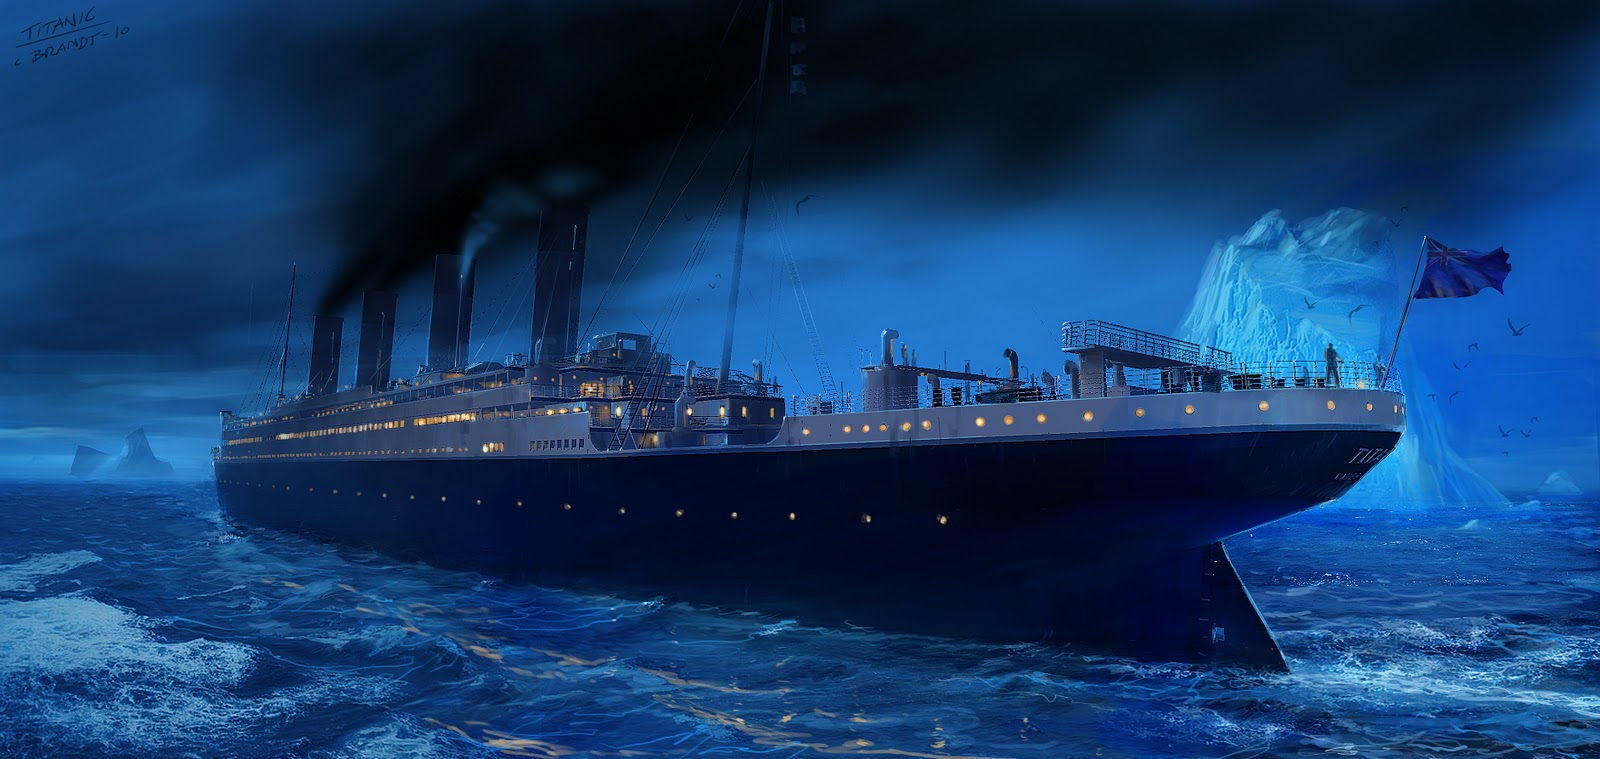
\includegraphics[scale = .15]{titanic.jpg}
\end{center}
\begin{itemize}
\item In 1912, the Titanic sank after colliding with an iceberg
\item Total number of passengers and crew: 2224
\begin{itemize}
\item How many people survived? \pause 722
\end{itemize}
\item Kaggle: Can we predict which passengers survived?
\end{itemize}
\end{frame}

\begin{frame}
\frametitle{The Data}
{\small train.csv:}
\begin{center}
{\tiny
\begin{tabular}{|r|r|r|l|r|r|r|r|r|l|}\hline
ID	& Surv.	& Cl	& Name					& S	& Age	& Sib/Sp	& Par/Ch	& Fare	& Port		\\\hline
1	& 0		& 3	& Braund, Owen			& M	& 22		& 1		& 0		& \$7.25	& Southampton	\\\hline
2	& 1		& 1	& Cumings, Florence		& F	& 38		& 1		& 0		& \$71.28	& Cherbourg	\\\hline
3	& 1		& 3	& Heikkinen, Laina			& F	& 26		& 0		& 0		& \$7.93	& Southampton	\\\hline
4	& 1		& 1	& Futrelle, Lily				& F	& 35		& 1		& 0		& \$53.10	& Southampton	\\\hline
5	& 0		& 3	& Allen, William			& M	& 35		& 0		& 0		& \$8.05	& Southampton	\\\hline
6	& 0		& 3	& Moran, James			& M	& NA		& 0		& 0		& \$8.46	& Queenstown	\\\hline
...	& ...		& ...	& ...						& ...	& ...		& ...		& ...		& ...		& ...			\\\hline
891	& 0		& 3	& Dooley, Patrick			& M	& 32		& 0		& 0		& \$7.75	& Queenstown	\\\hline
\end{tabular}
}
\end{center}
{\small test.csv:}
\begin{center}
{\tiny
\begin{tabular}{|r|r|r|l|r|r|r|r|r|l|}\hline
ID	& Surv.	& Cl	& Name					& S	& Age	& Sib/Sp	& Par/Ch	& Fare	& Port		\\\hline
892	& ?		& 3	& Kelly, James				& M	& 35		& 0		& 0		& \$7.83	& Queenstown	\\\hline
893	& ?		& 3	& Wilkes, Ellen				& F	& 47		& 1		& 0		& \$7.00	& Southampton	\\\hline
894	& ?		& 2	& Myles, Thomas\hspace{.25cm} & M& 62	& 0		& 0		& \$9.69	& Queenstown	\\\hline
...	& ...		& ...	& ...						& ...	& ...		& ...		& ...		& ...		& ...			\\\hline
1309	& ?		& 3	& Peter, Michael			& M	& NA		& 1		& 1		& \$22.36	& Cherbourg	\\\hline
\end{tabular}
}
\end{center}
\vspace{.5cm}
{\small Brainstorm: What features {\it might} make a person more likely to survive?}
\end{frame}

\begin{frame}
\frametitle{Method 1: $k$-Nearest Neighbors}
1-Nearest Neighbor: For each person in the test set,\\
\hspace{2.5cm} find the most similar person in the training set.\\~\\
2-Nearest Neighbors: For each person in the test set,\\
\hspace{2.5cm} find the 2 most similar people in the training set.\\~\\
3-Nearest Neighbors: For each person in the test set,\\
\hspace{2.5cm} find the 3 most similar people in the training set.\\
...\\~\\
$k$-Nearest Neighbors: For each person in the test set,\\
\hspace{2.5cm} find the $k$ most similar people in the training set.\\~\\~\\
How do we define similarity?
\end{frame}

\begin{frame}
\frametitle{$k$-Nearest Neighbors on a toy data set}
\begin{center}
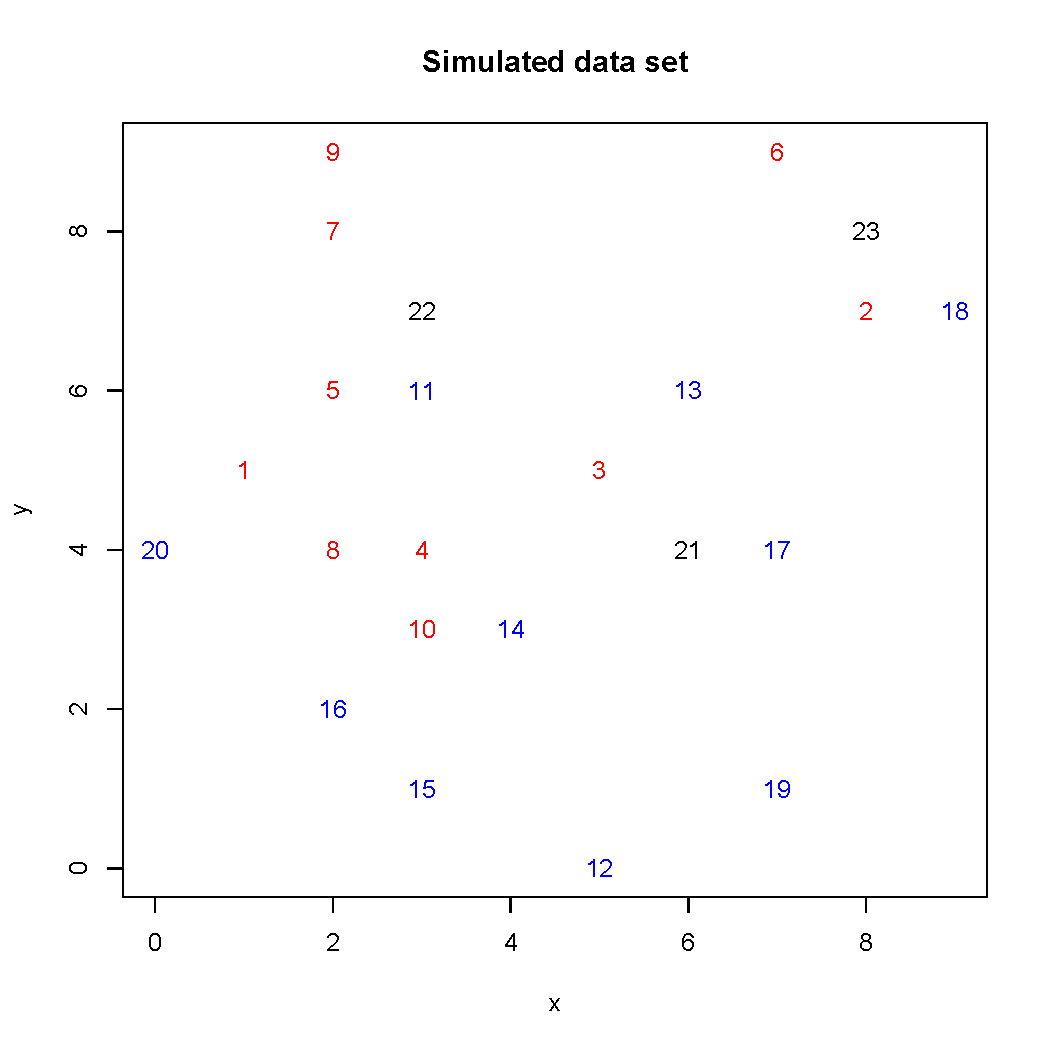
\includegraphics[scale=0.4]{plot.pdf}
\end{center}
\end{frame}

\begin{frame}
\frametitle{$k$-Nearest Neighbors on Titanic data}
\end{frame}

\begin{frame}
\frametitle{Method 2: Linear Regression}
\end{frame}

\begin{frame}
\frametitle{Method 3: Logistic Regression}
\end{frame}

\begin{frame}
\frametitle{Method 4: Linear Discriminant Analysis}
\end{frame}

\begin{frame}
\frametitle{Method 5: Quadratic Discriminant Analysis}
\end{frame}

\begin{frame}
\frametitle{Method 6: Support Vector Machines}
\end{frame}

\end{document}